
\section{Joint Conceptualization}
In this section, we present our solution to estimate $ P(\langle c_1,c_2 \rangle | \langle e_1,e_2\rangle) $.
Our basic idea is considering the conceptualization of $e_1$ and $e_2$ jointly instead of independently.
By joint conceptualization, we derive a new optimization objective function.


\paragraph{Estimation of $P(\langle c_1,c_2\rangle | \langle e_1,e_2\rangle)$ }
A straightforward estimation of $P( \langle c_{1},c_{2} \rangle | \langle e_{1},e_{2} \rangle )$ is as Eq~\ref{eq:naive} when we assume that the choice of concept for $e_1$ is independent of that for $e_2$.
\begin{equation}
\label{eq:naive}
\small
\begin{split}
P(\langle c_{1},c_{2}\rangle |\langle e_{1},e_{2} \rangle) = P(c_1|e_1) P(c_2|e_2)
\end{split}
\end{equation} The rationality is that the typicality of a concept pair can be quantified as the product of their respective typicality of each concept given its corresponding entity.
However, the assumption does not always hold as shown in Example~\ref{exa:jc}. Hence, we need to introduce a factor $\alpha(c_1,c_2)$ into Eq.~\ref{eq:target_expand2_jr} to quantify {\it how likely that the two concepts are the appropriate concepts of the attribute}. Thus, we have the following improved estimation:
\begin{equation}
\label{eq:target_expand2_jr}
\small
\begin{split}
P(\langle c_{1},c_{2}\rangle |\langle e_{1},e_{2} \rangle) = \alpha(c_1,c_2)  P(c_1|e_1)  P(c_2|e_2)
\end{split}
\end{equation}


One simple estimation of $\alpha(c_1,c_2)$ is using the prior probability of $\langle c_1, c_2\rangle$, i.e., $P(\langle c_1,c_2\rangle)$ (see Eq.~\ref{eq:rel_jdp}).
\begin{equation}\label{eq:rel_jdp}
\small
  \alpha(c_1,c_2) = P(\langle c_1, c_2\rangle)
\end{equation}
This is reasonable since the true concept pair for an entity pair in general has a larger probability than
a false concept pair.

Using Bayesian rules, $P(a| \langle c_{1},c_{2} \rangle )$ can be restated by the following equation:
\begin{equation}
\label{eq:target_expand1}
\small
P(a|\langle c_{1},c_{2} \rangle)= \frac{ P(\langle c_{1},c_{2}\rangle|a)P(a) }{ P(\langle c_{1},c_{2}\rangle) }
\end{equation},
where $P(a)$ is probability to observe an entity pair with attribute $a$.
Thus the objective function is reduced to Eq.~\ref{eq:simple_obj} when Eq.~\ref{eq:rel_jdp} holds.
\begin{equation}
\label{eq:simple_obj}
\small
 \argmax_a \sum_{c_i\in C_1, c_j\in C_2} P(\langle c_{i},c_{j}\rangle |a) P(a) P(c_i|e_1) P(c_j|e_2)
\end{equation}




\nop{
\subsection{Target Expand}
Given, Eq~\ref{eq:target}, the estimation of $P(a| \langle e_1,e_2 \rangle )$ boils down to 2 parts:
\begin{enumerate}
\item $P(a| \langle c_{1},c_{2} \rangle )$:  the typicality of an attribute for a concept pair.
\item $P( \langle c_{i},c_{j} \rangle | \langle e_{1},e_{2} \rangle )$:  the typicality of the concept pair for an entity pair.
\end{enumerate}

Using Bayesian rules, $P(a| \langle c_{1},c_{2} \rangle )$ can be restated in Eq.\ref{eq:target_expand1}:
\begin{equation}
\label{eq:target_expand1}
\begin{split}
P(a|\langle c_{1},c_{2} \rangle) &= \frac{ P(\langle c_{1},c_{2}\rangle|a)\times P(a) }{ P(\langle c_{1},c_{2}\rangle) }
%&=\frac{ p((c_{1},c_{2})|a)\times P(a) }{ \sum{P( (c_{1},c_{2})|a^* )\times P(a^*)   } },
\end{split}
\end{equation},
where $P(a)$ is probability to observe an entity pair with attribute $a$.
}

\subsection{Solution Framework}
Now we are ready to present our framework. The main framework is illustrated in Figure~\ref{fig:framework}, which consists of two major components: {\it online computation} and {\it offline training}. 
We refer to our system as \ac{Entity Relation Finder (ERF)}.
ERF takes an entity pair as input and find its most plausible relation as the result.
As a preprocessing step, we first directly lookup the attribute for the query entity pair from DBpedia.
If DBpedia has SPO triples connecting the entity pair, we direct return the predicate as the answer.
Otherwise, the procedure goes into the online computation component.
The online component calculates $ P(a|  \langle e_1,e_2 \rangle  )$ for each candidate attribute in $A$ (the set of all attributes) by Eq.~\ref{eq:simple_obj} and return the maximal one as the answer attribute. To compute Eq.~\ref{eq:simple_obj}, we need to compute $P(\langle c_1,c_2 \rangle |a)$, $P(a)$, $P(c_1|e_1)$ and $P(c_2|e_2)$. 

In the online part, we compute $P(c_1|e_1)$ and $P(c_2|e_2)$ on demand instead of materializing them. Because we only conceptualize an entity into its head concept and the conditional probability of head concept cannot be carefully recaculated. In general, a materialization suffers from quadratic complexity, which is unaffordable when we have millions of entities. We will elaborate it later in head-aware conceptualization section.
In the offline part, we compute $P(c_1,c_2|a)$ and $P(a)$ by leveraging the SPO triples in DBpedia and isA relationships in $Probase$. 
We elaborate the detail in the next section.





\begin{figure}[!t]
\vspace{-4mm}
\centering
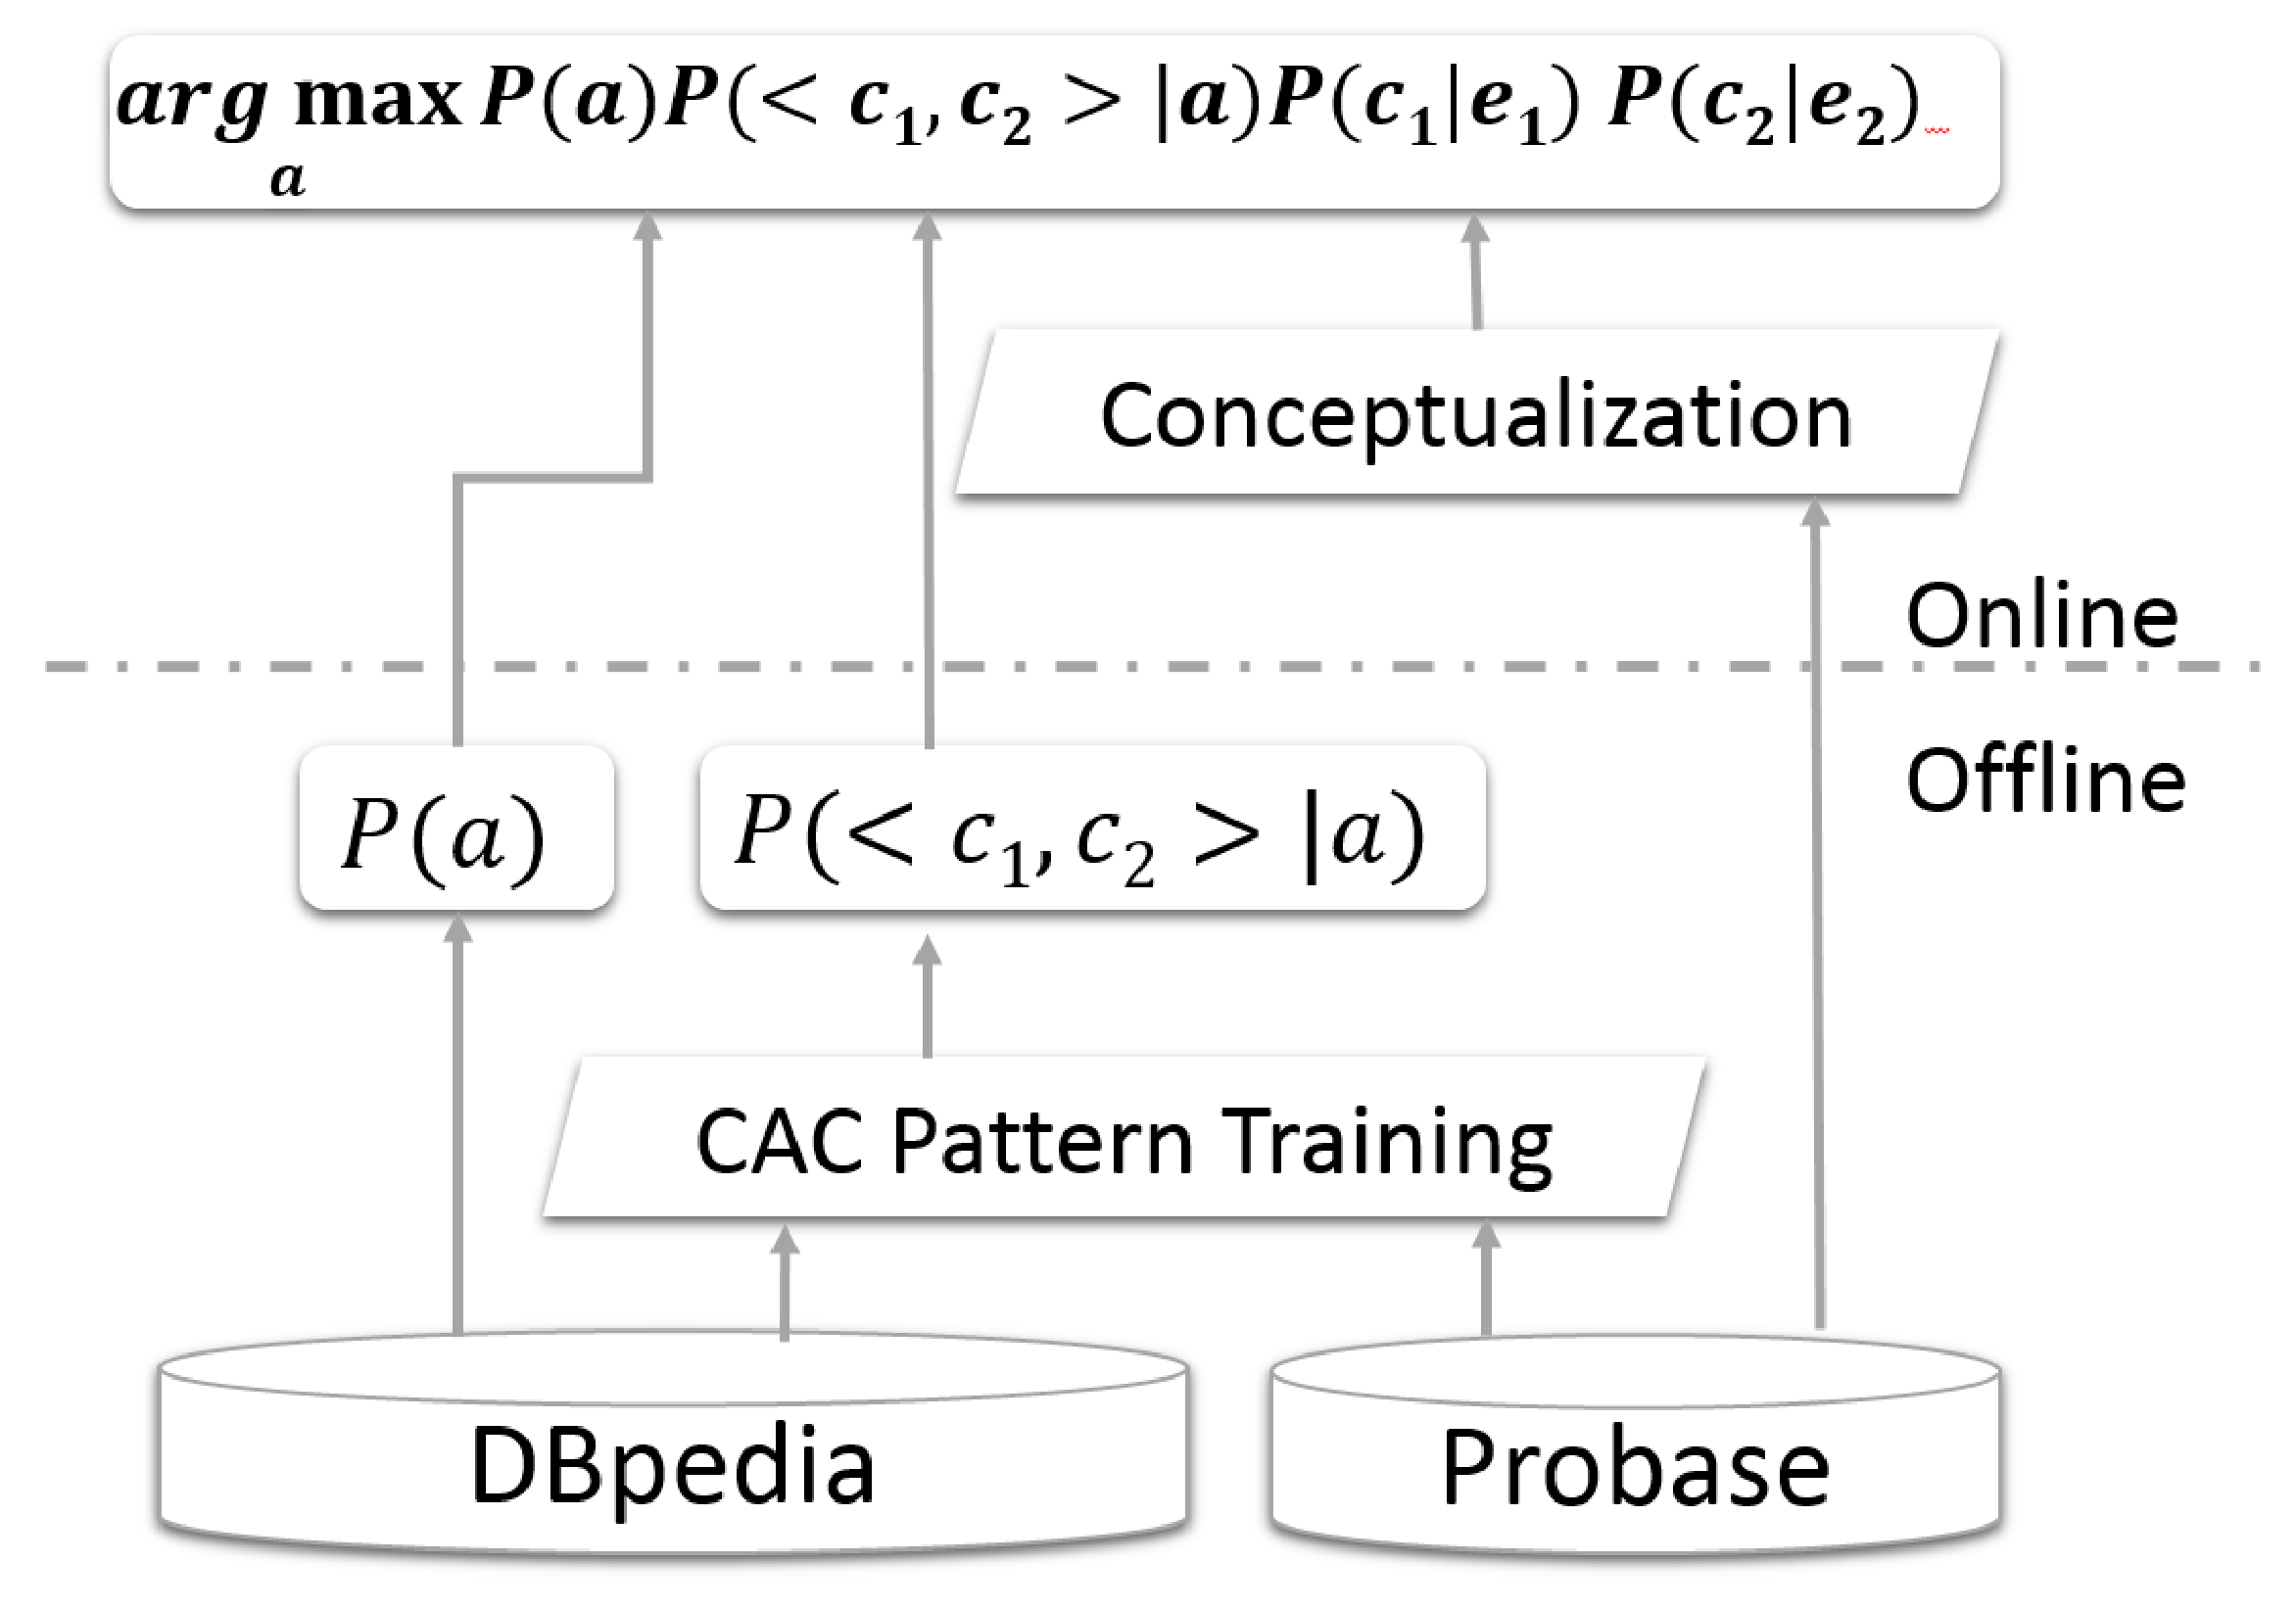
\epsfig{file=resources/framework.eps,width=0.8\columnwidth,height=0.5\columnwidth}
\vspace{-4mm}
\caption{System Framework of ERF}
\label{fig:framework}
\vspace{-6mm}
\end{figure}


\nop{
In the online part, we first directly lookup the attribute for the query entity pair from DBpedia.
If DBpedia has no the exact the SPO triples connecting the entity pair, we In $step 2$, the concepts of the entities in knowledge bases are calculated(i.e. $P(c_i|e_i)$ in Eq.~\ref{eq:target_expand2_jr}).
The detailed process in in
$Step 3$ is the training process, $P( \langle c1,c2 \rangle ,a)$ is calculated for every attribute $a$ in Eq.~\ref{eq:pccga}.
The result is then stored in Concept Relation DB in $step 4$.

In  $step 1$, when a query entity pair comes, knowledge bases such as DBpedia are looked up and the exact relationship, if exists, is answered in the first place.
If nothing is found in $step 1$, the process will go into the ERF solution.

We first conceptualize the 2 entities in $step 2$.
The concept similarity score in Eq.~\ref{eq:target_expand2_jr}) is retrieved from the Concept Relation DB in $4$.
%\ref{eq:pcca}
So far we get everything for calculating Eq.~\ref{eq:target_expand2_jr}).
Then in $step 7$ we query the concept relation database and get the relation between concept pairs, specifically, $P(a| \langle c_1,c_2 \rangle )$ in Eq.~\ref{eq:target_expand1}.
Finally, we achieve the final object by combining all these together to infer $\argmax P(a| \langle e_1,e_2 \rangle )$ from Eq.~\ref{eq:target_expand_all}.
We return the the attribute owning the maximal score as the explanation for the relationship between the entity pair.

When no direct edges are found, we use the shortest path on the concept attribute graph to find the middle concepts, then the problem automatically reduced to relation explanation of several pairs of entities, discussing which is beyond the coverage of this paper.
}


%\paragraph{Paper Orgnization}
%The rest of the paper is organized as follows, Section~\ref{sec:conceptualization} describe how to derive $P(c|e)$ leveraging the \xch{basicness} of concept, Section~\ref{sec:fafa} is devoted to the offline calculation of $JD(c_1,c_2)$ and $P((c_{1},c_{2})|a)$.
%\renewcommand\baselinestretch{-6}\selectfont
\renewcommand{\arraystretch}{-2}
%
%\begin{table}[htbp]
%  \centering
%     \small
%  \caption{Notation Table}
%    \footnotesize
%
%    \begin{tabular}{|ll|ll|}
%    \hline
%    notation                            &  meaning                            & notation                            &  meaning  \\
%    \hline
%    $n(\cdot)$                          &  count of                            & $e_i$                               &  entity  \\
%    $h(\cdot)$                          &  head of                             & $c_i$                               &  concept  \\
%    $a$                                 &  attribute                          & $c_l$                               &  long concept  \\
%    $\bar{C}$                           &  head concept set                  & $c_h$                               &  head concept  \\
%    $\langle e_1,e_2\rangle$            &  entity pair                        & $\langle c_1,c_2\rangle$            &  concept pair \\
%    $\alpha(\cdot,\cdot)$               &  joint factor                       & $T_k$                               & \parbox{0.26\columnwidth}{ set of E$A$E tuple with $a_k$ as $A$} \\
%    \parbox{0.15\columnwidth}{\scriptsize $P(a|\langle c_{1},c_{2}\rangle)$ }  &  \parbox{0.24\columnwidth}{ the typicality of an attribute for a concept pair. }& \parbox{0.23\columnwidth}{\scriptsize $P(\langle  c_{i},c_{j}\rangle|\langle e_{1},e_{2}\rangle)$} & \parbox{0.26\columnwidth}{ the typicality of the concept pair for an entity pair} \\
%    \hline
%
%    \end{tabular}%
%
%  \label{tab:notation}%
%  \vspace{-6mm}
%\end{table}%
%
%\renewcommand{\arraystretch}{1}

%First,we do conceptualization.
%
%Next,Judge whether the 2 entities are conceptually same
%
%Then, there are 2 cases of the CanBeExplained function:
%
%\begin{itemize}
%\item Explain 2 conceptually similar entity
%
%\begin{table}[htbp]
%  \centering
%  \caption{conceptually similar entity}
%    \begin{tabular}{rr}
%    \toprule
%    entity & concept \\
%    \midrule
%    Steve jobs & Person \\
%    Bill Gates & Person \\
%    \bottomrule
%    \end{tabular}%
%  \label{tab:addlabel}%
%\end{table}%
%
%
%\item Explain 2 conceptually different entity
%% Table generated by Excel2LaTeX from sheet 'Sheet1'
%\begin{table}[htbp]
%  \centering
%  \caption{Add caption}
%    \begin{tabular}{rr}
%    \toprule
%    entity & concept \\
%    \midrule
%    Mona Lisa & Painting \\
%    Renaissance & Period \\
%    \bottomrule
%    \end{tabular}%
%  \label{tab:addlabel}%
%\end{table}%
%
%Note that the concept here are not unique.
%
%\end{itemize}
%
%
%Last, We rank all the explanations in each step.
%
%
%

